\documentclass[tikz,border=5pt]{standalone}
\usepackage{tikz}
\usetikzlibrary{positioning, arrows.meta, calc}

\begin{document}
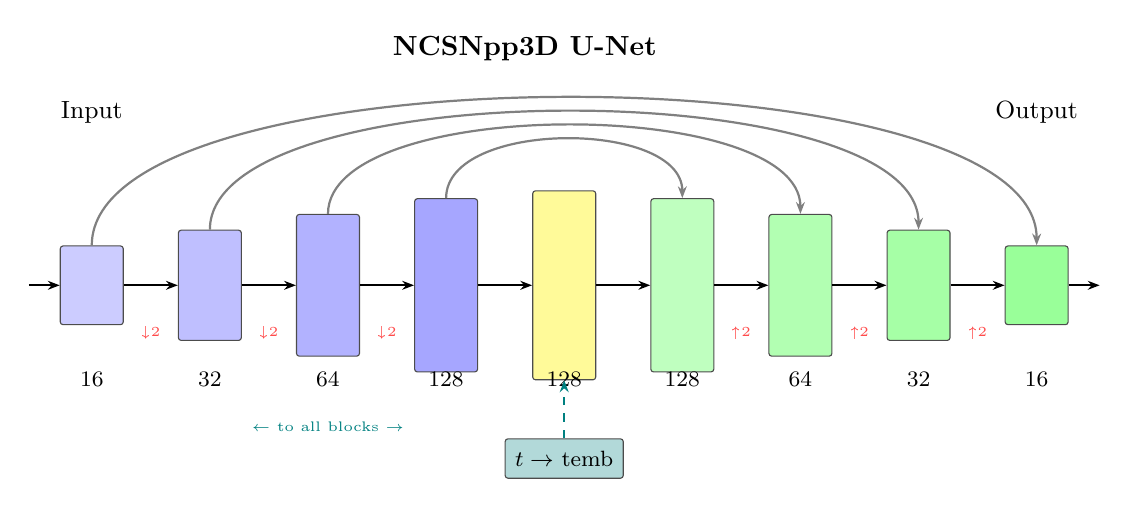
\begin{tikzpicture}[
    block/.style={rectangle, draw=black!70, fill=#1, minimum width=0.8cm, rounded corners=1pt, font=\footnotesize},
    arrow/.style={-{Stealth[length=1.5mm]}, thick},
    skip/.style={-{Stealth[length=1.5mm]}, thick},
    label/.style={font=\small},
]

% Title
\node[label, font=\bfseries] at (5.5, 3) {NCSNpp3D U-Net};

% Encoder blocks (increasing height = more channels)
\node[block=blue!20, minimum height=1.0cm] (e1) at (0, 0) {};
\node[block=blue!25, minimum height=1.4cm] (e2) at (1.5, 0) {};
\node[block=blue!30, minimum height=1.8cm] (e3) at (3, 0) {};
\node[block=blue!35, minimum height=2.2cm] (e4) at (4.5, 0) {};

% Middle (bottleneck)
\node[block=yellow!40, minimum height=2.4cm] (mid) at (6, 0) {};

% Decoder blocks (decreasing height)
\node[block=green!25, minimum height=2.2cm] (d4) at (7.5, 0) {};
\node[block=green!30, minimum height=1.8cm] (d3) at (9, 0) {};
\node[block=green!35, minimum height=1.4cm] (d2) at (10.5, 0) {};
\node[block=green!40, minimum height=1.0cm] (d1) at (12, 0) {};

% Input/Output labels
\node[label] at (0, 2.2) {Input};
\node[label] at (12, 2.2) {Output};

% Channel labels (below blocks)
\node[font=\footnotesize] at (0, -1.2) {16};
\node[font=\footnotesize] at (1.5, -1.2) {32};
\node[font=\footnotesize] at (3, -1.2) {64};
\node[font=\footnotesize] at (4.5, -1.2) {128};
\node[font=\footnotesize] at (6, -1.2) {128};
\node[font=\footnotesize] at (7.5, -1.2) {128};
\node[font=\footnotesize] at (9, -1.2) {64};
\node[font=\footnotesize] at (10.5, -1.2) {32};
\node[font=\footnotesize] at (12, -1.2) {16};

% Horizontal arrows (data flow)
\draw[arrow] (-0.8, 0) -- (e1.west);
\draw[arrow] (e1.east) -- (e2.west);
\draw[arrow] (e2.east) -- (e3.west);
\draw[arrow] (e3.east) -- (e4.west);
\draw[arrow] (e4.east) -- (mid.west);
\draw[arrow] (mid.east) -- (d4.west);
\draw[arrow] (d4.east) -- (d3.west);
\draw[arrow] (d3.east) -- (d2.west);
\draw[arrow] (d2.east) -- (d1.west);
\draw[arrow] (d1.east) -- (12.8, 0);

% Skip connections (curved, from top)
\draw[skip, gray] (e4.north) .. controls ++(0, 1) and ++(0, 1) .. (d4.north);
\draw[skip, gray] (e3.north) .. controls ++(0, 1.5) and ++(0, 1.5) .. (d3.north);
\draw[skip, gray] (e2.north) .. controls ++(0, 2) and ++(0, 2) .. (d2.north);
\draw[skip, gray] (e1.north) .. controls ++(0, 2.5) and ++(0, 2.5) .. (d1.north);

% Downsample indicators (red triangles pointing right)
\node[font=\tiny, red!70] at (0.75, -0.6) {↓2};
\node[font=\tiny, red!70] at (2.25, -0.6) {↓2};
\node[font=\tiny, red!70] at (3.75, -0.6) {↓2};

% Upsample indicators
\node[font=\tiny, red!70] at (8.25, -0.6) {↑2};
\node[font=\tiny, red!70] at (9.75, -0.6) {↑2};
\node[font=\tiny, red!70] at (11.25, -0.6) {↑2};

% Time embedding (below)
\node[block=teal!30, minimum height=0.5cm, minimum width=1.5cm] (temb) at (6, -2.2) {\footnotesize $t \to$ temb};
\draw[arrow, teal, dashed] (temb.north) -- (mid.south);
\node[font=\tiny, teal] at (3, -1.8) {$\leftarrow$ to all blocks $\rightarrow$};

\end{tikzpicture}
\end{document}
